Today's data are shown in Fig. \ref{fig:todays-data}, and yesterday's
data are shown in Fig. \ref{fig:yesterdays-data}.

\begin{figure}[htbp]
\centering
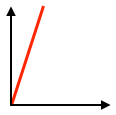
\includegraphics{img/todays-data.png}
\caption{Today's \(y=mx+b\) data.\label{fig:todays-data}}
\end{figure}

\begin{figure}[htbp]
\centering
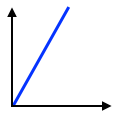
\includegraphics{img/yesterdays-data.png}
\caption{Yesterday's \(y=mx+b\) data.\label{fig:yesterdays-data}}
\end{figure}

Earlier data are shown in Fig. \ref{fig:earlier-data}. Fig.
\ref{fig:earlier-data}a is for two days ago and Fig.
\ref{fig:earlier-data}b is for three days ago.

\begin{figure}[htbp]
\centering
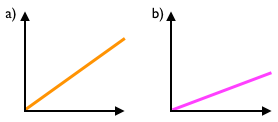
\includegraphics{img/earlier-data.png}
\caption{Data from a) two days ago, and b) three days
ago.\label{fig:earlier-data}}
\end{figure}

Figures \ref{fig:todays-data}--\ref{fig:earlier-data}
(\ref{fig:todays-data},\ref{fig:yesterdays-data},\ref{fig:earlier-data})
reveal an increasing slope with time.
